\section{Proste testy}

Dla zaprezentowania działania algorytmów SocialPageRank i Adapted PageRank przeprowadzono obliczenia na prostych danych. Wszystkie obliczenia wykonano używając danych podanych w tabeli \ref{fig:test_proste_dane}. 


\begin{figure}[htb]
  \centering
  \begin{tabular}{|c|c|c|c|c|}
    \hline
    \multicolumn{1}{|c|}{}&\multicolumn{2}{c|}{Użytkownicy}\\

    \cline{2-3}
    \multicolumn{1}{|c|}{}&użytkownik 1&użytkownik 2\\
    \hline
 	http://www.ted.com/ & inspiration & \\
	http://www.colourlovers.com/&	design & inspiration \\
	http://www.behance.net/	&portfolio, design & portfolio, inspiration \\
    \hline
  \end{tabular}
  \caption{Dane do prostych testów}
  \label{fig:test_proste_dane}
\end{figure}

\section{SocialPageRank: wyniki}

\subsection{Wyniki algorytmu dla prostych danych}

W tabelce \ref{fig:test_proste_dane} znajdują się dane, dla których zostało sprawdzone działanie algorytmu Social PageRank. Dane są nie duże i składają się z trzech różnych dokumentów, dwóch użytkowników i trzech tagów.

\begin{figure}
  \centering
  \begin{tabular}{|c|c|c|c|c|}
    \hline
    \multicolumn{1}{|c|}{}&\multicolumn{2}{c|}{Użytkownicy}\\

    \cline{2-3}
    \multicolumn{1}{|c|}{}&użytkownik 1&użytkownik 2\\
    \hline
 	http://www.ted.com/ & inspiration & \\
	http://www.colourlovers.com/&	design & inspiration \\
	http://www.behance.net/	&portfolio, design & portfolio, inspiration \\
    \hline
  \end{tabular}
  \caption{Dane do prostych testów}
  \label{fig:test_proste_dane}
\end{figure}

Dla takich danych macierz $M_{d,u}$ mówiąca o zależności dokumentów z użytkownikami ma postać:

\[
 M_{d,u} =
 \begin{pmatrix}
  1 & 0 \\
  1 & 1 \\
  1 & 2
 \end{pmatrix}
\]

Macierz użytkowników i tagów, $M_{u,t}$:

\[
 M_{u,t} =
 \begin{pmatrix}
  1 & 1 & 1 \\
  2 & 0 & 1 
 \end{pmatrix}
\]

Macierz tagów i dokumentów, $M_{t,d}$:
\[
 M_{t,d} =
 \begin{pmatrix}
  1 & 1 & 1 \\
  0 & 1 & 1 \\
  0 & 0 & 2 
 \end{pmatrix}
\]


\subsection*{wyniki:}
Dla powyższych danych wyniki algorytmu zbiegają po czterech iteracjach z dokładnością
$|P_3 - P_4|  < 10^{-10}$. Wyniki zostały przedstawione w tabelce \ref{fig:social_page_simple_wyniki}


\begin{table}[h]
  \centering
    \begin{tabular}{ | c | c | }
\hline
&Social PageRank \\
\hline
www.ted.com & 0.2381373691295440 \\
www.colourlovers.com  & 0.4343479235414989 \\
www.behance.net & 0.8686958470829979 \\
\hline
\end{tabular}
  \caption{Wyniki działania algorytmu Social PageRank}
  \label{fig:social_page_simple_wyniki}
\end{table}


Można zauważyć, że największy ranking ma strona behance.net, która została dodana przez dwóch użytkowników i oznaczonych najpopularniejszymi tagami - 2 razy tagiem portfolio, użytym tylko dla tej strony, raz tagiem design, który użyty był 2 razy w powyższych danych i również raz tagiem inspiration, który jest najpopularniejszym tagiem, użytym w przykładzie aż 3 razy. 












\section{Wyniki algorytmu Adapted PageRank dla prostych danych}


Algorytm Adapted PageRank przetestowano na tych samych danych co algorytm SocialPageRank (tabelka \ref{fig:test_proste_dane}). Macierz asocjacyjna powstała z tych danych ma wymiary $8 \times 8$ i wygląd:

\[
 G_f =
 \begin{pmatrix}
0 & 0 & 0 & 1	 & 0 & 1 & 0 & 0\\
0 & 0 & 0 & 1 & 1 & 1 & 1 & 0\\
0 & 0 & 0 & 2 & 2 & 1 & 1 & 2\\
1 & 1 & 2 & 0 & 0 & 1 & 2 & 1\\
0 & 1 & 2 & 0 & 0 & 2 & 0 & 1\\
1 & 1 & 1 & 1 & 2 & 0 & 0 & 0\\
0 & 1 & 1 & 2 & 0 & 0 & 0 & 0\\
0 & 0 & 2 & 1 & 1 & 0 & 0 & 0
 \end{pmatrix}
\]

\begin{table}[h]
  \centering
    \begin{tabular}{ | c | c | }
\hline
&Adapted PageRank \\
\hline
doc: http://www.ted.com/ & 0.280676409730572 \\
doc: http://www.colourlovers.com/ & 0.369220441236174 \\
doc: http://www.behance.net/ & 0.384551423972747 \\
\hline
usr: użytkownik A & 0.402473669662513 \\
usr: użytkownik B & 0.354578057974890 \\
\hline
tag: inspiration & 0.383291185401107 \\
tag: design & 0.321455285546253 \\ 
tag: portfolio	 & 0.314739469615726 \\
\hline
\end{tabular}
  \caption{Wyniki działania algorytmu Adapted PageRank}
  \label{fig:adapted_page_simple_wyniki}
\end{table}

Zbierzność wektora została uzyskana po 22 iteracjach. Jest to zdecydowanie dłuższy czas w porównaniu z czterema wymaganymi iteracjami przy poprzenim algorytmie


Analizując wyniki z tabeli \ref{fig:test_proste_dane} można zauważyć, że kolejność stron według obydwu algorytmów jest taka sama. Najwyższy ranking wśród dokumentów ma również strona behence.net, a najniższy strona ted.com. 

Porównując wyniki algorytmów Adapted PageRank i SocialPageRank można zauważyć różnice miedzy poszczególnymi wartościami. Dla przykładu, różnica miedzy pierwszym a drugim dokumentem jest bardzo mała w porównaniu z prawie dwa razy większą wartością uzyskaną przy pomocy algorytmu Social PageRank. Ponieważ strony różnią się tym, że zostały opisane różna ilością tagów można po tym wywnioskować ze nadanie większej ilości tagów nie ma dużego wpływu na ranking strony. Za to zmniejszenie liczby użytkowników którzy tą stronę dodali bardzo zmniejsza wynik.





\section{Wyniki działania algorytmów}

W tablicach \ref{tab:adapted_wyniki_sorted} i \ref{tab:social_page_wyniki_sorted} przedstawiono rezultaty działania algorytmów SocialPageRank, AdaptedPageRank. Wyniki te zostały posortowane w zależności od wyniku algorytmu SocialPageRank \ref{tab:social_page_wyniki_sorted} i  AdaptedPageRank \ref{tab:adapted_wyniki_sorted}. Dodatkowo w tablicy \ref{tab:inne_wyniki_sorted} znajdują się wyniki posortowane w zależności od sumy popularności dokumentów w sieciach twitter, facebook i digg. Można zauważyć, że żaden z pierwszych 25 dokumentów się nie pokrywa. 

W tablicy \ref{tab:rozne_wyniki}  znajdują się wartości maksymalne, minimalne i średnie dla różnych algorytmów. Można zauważyć, że podobnie jak dla prostych przykładów, algorytm AdaptedPageRank ma zdecydowanie mniejsze różnice miedzy poszczególnymi wynikami. 


\begin{table}[htb]
  \centering
    \begin{tabular}{ | l | l | l | l| }
\hline
  & maksymalna & średnia & minimalna \\
\hline
SocialPageRank    &  59.9655565  & 0.654392541 &  1.4996654e-012 \\
AdaptedPageRank &   0.7196510  & 0.497870340 &  0.2520965 \\
inne            & 578287638         & 17132.4861 (21544.9729)   & 0 \\
\hline
\end{tabular}
  \caption{ Maksymalne, średnie, minimalne wartości algorytmów. }
  \label{tab:rozne_wyniki}
\end{table}


Dokładniej zelażnością między poszczególnymi wynikami można się przyjrzeć na rysunkach \ref{fig:social-adapted}, \ref{fig:adapted-social}, \ref{fig:adapted-inne}, \ref{fig:social-inne}. Na wykresach tych przedstawiono wyniki algorytmów posortowane po jednej z danych. Dodatkowo na rysunku \ref{fig:adapted-inne} i \ref{fig:social-inne} znajdują się wyniki odpowiednio algorytmu AdaptedPageRank i SocialPageRank przedstawione razem z danymi uzyskanymi z innych sieci społecznościowych. Na \ref{fig:social-inne} można zaobserwować zależność między wynikami algorytmu SocialPageRank a popularnością danych dokumentów w innych sieciach społecznościowych.



\begin{figure}[htbp]

    \centering
    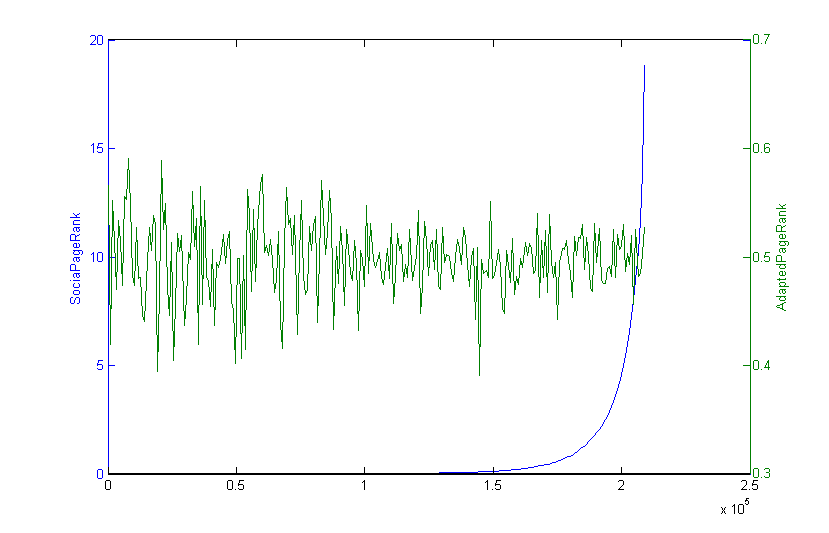
\includegraphics[width=\linewidth]{social-adapted.png}
    \caption{Zależności między wynikami algorytmów SocialPageRank i AdaptedPageRank. Posortowane po wartościach algorytmu SocialPageRank}
    \label{fig:social-adapted}
\end{figure}

\begin{figure}[htbp]
    \centering
    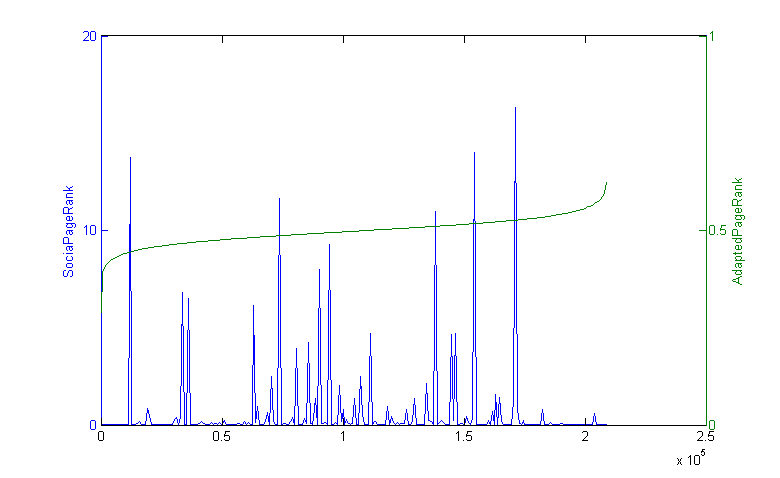
\includegraphics[width=\linewidth]{adapted-social.png}
    \caption{Zależności między wynikami algorytmów SocialPageRank i AdaptedPageRank. Posortowane po wartościach algorytmu AdaptedPageRank}
    \label{fig:adapted-social}

\end{figure}



\begin{figure}[htbp]

    \centering
    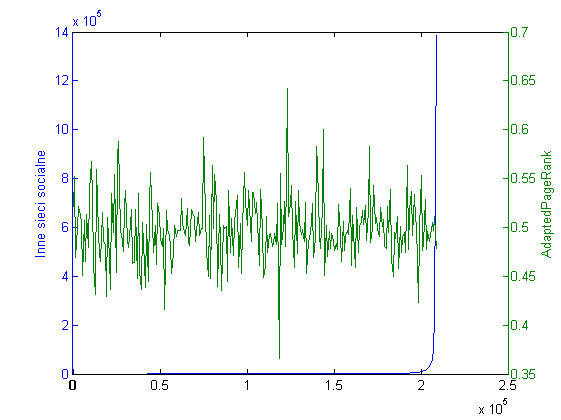
\includegraphics[width=\linewidth]{adaoted-inne.png}
    \caption{Zależności między wynikami algorytmów AdaptedPageRank i danymi z innych sieci socialnych. Posortowane po wartościach z innych sieci}
    \label{fig:adapted-inne}
\end{figure}

\begin{figure}[htbp]
    \centering
    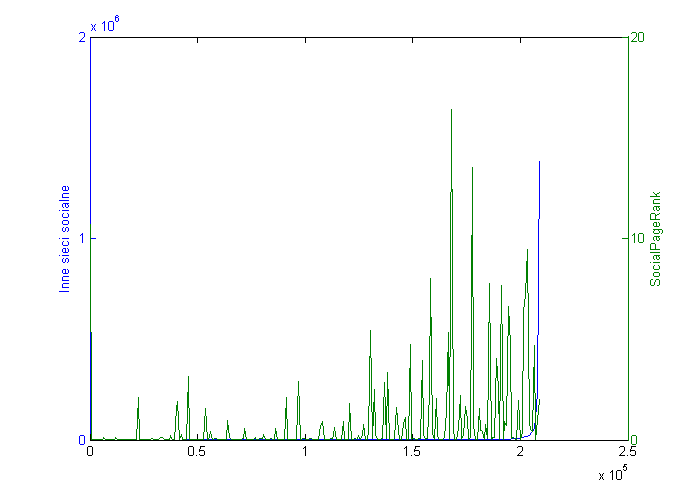
\includegraphics[trim = 0mm 10mm 0mm 0mm, width=\linewidth]{social-inne.png}
    \caption{Zależności między wynikami algorytmów SocialPageRank i danymi z innych sieci socialnych. Posortowane po wartościach z innych sieci}
    \label{fig:social-inne}

\end{figure}
















